\documentclass[parskip=no,12pt,a4paper,twoside,headings=openright]{scrreprt}
% switch to scrbook if you want roman page numbers for the front matter
% however scrbook has no 'abstract' environment!
% if your thesis is in english, use "parskip=no" instead

% binding correction (BCOR) von 1cm für Leimbindung
\KOMAoptions{BCOR=1cm}
\KOMAoptions{draft=yes}

\usepackage[utf8]{inputenc} % encoding of sources
\usepackage[T1]{fontenc}
\usepackage{style/studarbeit}
\graphicspath{{img/}{fig/}{style/}}

\title{Bounding Information Leakage by Combining an Interpreter with Model Counting}
\author{Tina Maria Strößner}
\thesistype{Masterarbeit}
\zweitgutachter{Prof.~Dr.~rer.~nat.~Bernhard~Beckert}
\betreuer{M.~Sc.~Johannes Bechberger  \& M.~Sc.~Simon Bischof}

\coverimage{img/4665389330_d09f3d6b75_z.jpg}
\abgabedatum{{\year=2021 \month=8 \day=9 \today}}

\newcommand{\libFIRM}{lib\textsc{Firm}}

\begin{document}

\begin{otherlanguage}{ngerman} % Titelseite ist immer auf Deutsch
\mytitlepage
\end{otherlanguage}

\begin{abstract}
\begin{center}\Huge\textbf{\textsf{Abstract}}
\end{center}
\vfill
\end{abstract}

\tableofcontents

\chapter{Introduction}\label{sec:intro}

\section{Motivation}

In February 2017, the American web services and web security company Cloudflare made headlines, when a security bug was discovered in an HTML parser. A buffer overrun caused the servers to leak sensitive data, such as browser cookies, authentication tokens or HTTP post bodies. The so-called `Cloudbleed' bug is one of many examples of software revealing secret data to unauthorized users, a security threat that has become more severe, as more and more software is used in the handling of sensitive data \cite{cloudbleedIssue, cloudbleedReport}. 

Qualitative information flow control aims to guarantee, that a program's public outputs are not influenced by secret its secret inputs, thus a malicious attacker has no possibility of obtaining secret information, by merely observing the program's outputs. This property is called \emph{non-interference}. 

For non-interferent programs, the secret inputs are guaranteed to have no influence on the public outputs, so unintentional data leaks are impossible. However, often this requirement is too strict for practical use. Consider the program shown in figure \ref{fig:pwChecker}. While the secret password is not leaked in its entirety, an attacker can gather some information by observing whether their guess was correct. Hence, non-interference is not given, however for most practical purposes, the information leakage from the password checker example would be fully acceptable and often also inevitable for the program's intended usage.

The desire to make information flow control applicable to more practical applications gave rise to the notion of quantitative information flow control (QIFC), where the amount of leakage in a program is measured in bits and compared to a predetermined limit. The amount of leakage in the password checker example is one bit.

\begin{figure}
\centering
\begin{minipage}{.7\linewidth}
    \begin{algorithm}[H]
        \begin{algorithmic}[1]
    \Procedure{check_password}{guess: int}
            \If{$guess == password$}
                \State $match \leftarrow 1$
            \Else
                \State $match \leftarrow 0$
            \EndIf\\
            \Return match
            \EndProcedure
    \end{algorithmic} 
    \end{algorithm}
    \end{minipage}
    \caption{Password Checker}
    \label{fig:pwChecker}
\end{figure}

QIFC analyses can typically be divided into 2 categories:

\emph{Static} analyses are performed without executing the program and rely solely on examination of the source code. Such analyses are sound in that they deliver an upper bound for the amount of information a program might leak. However, depending on the program, the upper bound the analysis is able to compute might be much larger than the actual leakage, due to the lack of knowledge about concrete control and data flows in the program.

Contrarily, \emph{dynamic} analyses compute a program's leakage by simulating one or more program executions. For these executions, dynamic analyses can compute a more precise estimation of the leakage than static analyses, however these estimations might not be a sound upper bound, since it is infeasible to analyse every possible input combination for the program.

\section{Related Work}\label{sec:relWork}

While early mentions of quantifying information flow have been made, for example by Denning \cite{denning82}, a formal definition and theoretical groundwork for the QIF problem are given more recently by Lowe \cite{lowe02} and Smith \cite{smith09}. A recent publication by Alvim et. al \cite{alvim19} gives a comprehensive overview over the theory behind quantitative information flow.

QIFC analyses based on model counting have previously been introduced by several people.
Newsome, McCamant and Song \cite{newsome09} transform their programs into boolean predicates that accurately models its semantics. Using SAT techniques they then measure the program's channel capacity. The results are used to find false positives in a dynamic taint analysis in order to more accurately determine the amount of influence of an attacker over the program.

Klebanov, Manthey and Muise (\cite{klebanov13}) use the bounded model checking tool CBMC (\cite{cbmc}) to generate a boolean predicate and the d-DNNF-based \#SAT tools \textsc{sharp}SAT (\cite{thurley06}) and \textsc{DSHARP} (\cite{muise12}).

A similar approach is used by Biondi et. al. in \cite{biondi18}. They also use CBMC to create a SAT formula. In order to address scalability issues with overly complex SAT formulas, they are the first use an approximate model counter, in this case ApproxMC (\cite{chakraborty13}).

Chu and Hashimoto in \cite{chu19} also combine the CBMC framework with an approximate model counter, however they do not measure channel capacity as the previously mentioned works did, instead they estimate the pre-image size of a certain program output.

A previous attempt at combining static and dynamic techniques has been made by McCamant and Ernst \cite{mccamant08}. They transform programs into network graphs with edge capacities corresponding to the amount of Information that might flow between the corresponding program parts. Thus, the maximum leak of information corresponds to the maximum flow in the created network. They use the approach to estimate the leakage of the input program, however their analysis is not sound and might underestimate leakage.

\pagebreak

In this thesis, we define and compare two different measures for information leakage: the first is one based on min-entropy and is used by many of the QIFC tools mentioned above. The second one is based on the notion of dynamic leakage during a single program run. We will present a model-counting based analysis that is able to provide estimations for both quantities.

Additionally, we present an integration of static QIF methods into our analysis in order to mitigate the difficulties, that other model counting based tools have.

The analysis will be integrated into an interpreter that provides the possibility of executing a program in an environment that can protect secret information by either aborting execution or masking values before they are leaked to a public channel.

\td{review -- especially last paragraph..}

\chapter{Theoretical Background}\label{sec:basics}

This chapter presents the theoretical background of this thesis. We will explain the foundations of quantitative information flow control and the different measures that are used to quantify information leakage. Furthermore, we will outline important aspects of (approximate) model counting, as well basic principles used in static (Q)IFC analyses \emph{Nildumu} and \emph{JOANA}, as both are used in our hybrid QIFC tool.

\section{Quantitative Information Flow Control}

Information flow control aims to guarantee the confidentiality of the secret input data of a program, by examining the flow of information through the program to public output channels, where the information would become accessible to an attacker.

There are different ways in which such information leakage might happen: Explicit information flows happen, when a secret values itself is written to a public channel or the information is copied to a variable that is later in leaked to a public channel. An example of a program is shown in figure \ref{fig:exEx}. Information leaks through implicit flows happen, when secret values affect the program's output through influencing the execution path. Figure \ref{fig:ifEx} shows a program snippet that contains an implicit flow. Additional to explicit and implicit flows, an attacker could gain information trough covert channels by observing a program's usage of different resources, such as time or memory \cite{smith07}.

Qualitative information flow analysis tries to prove the absence of explicit and implicit information flows, a property called \emph{non-interference}. For real world applications, leaking a certain amount of information is often required to build useful programs. In this case, the non-interference property is too strict. Instead, we wish to limit the amount of information that is leaked. Quantitative information flow analysis provides tools to measure how much information can be learned by an attacker about a program's secret inputs \cite{smith09}.

We consider the following scenario: Given a program \p, that accepts some input \In and produces some output \Out, how much information can an adversary \A learn about $H$, by observing \p and \Out?

\paragraph{Input program} We assume \p to be a sequential, deterministic program, that receives a set of inputs $\mathtt{H = \{h_1, ..., h_n\}}$ and produces a set of outputs $\mathtt{L = \{l_1, ..., l_m\}}$. We will write the sets of all possible inputs and outputs as $\mathcal{H}$ $\mathcal{L}$ respectively. Inputs are chosen based on a publicly known a priori probability distribution. The program text of \p is publicly known. A more detailed description of the input language we used, we refer to \ref{sec:inputLang}.

\paragraph{Security Lattice} Each element of \In and \Out is associated with an element of a security lattice, describing its confidentiality level. We use a lattice with two elements $\hat{l}$, for public values and $\hat{h}$ for secret values. If not otherwise specified, we consider all inputs to be high and all outputs to be low.
% Schneider -- nur high und low

\paragraph{Attacker Model} We consider an adversary \A that is able to observe the program text of \p and the resulting outputs on public channels. He or she is also aware of the set of program inputs and its underlying probability distribution. We assume the attacker is not able to extract any information through covert channels. The goal of the attacker is to guess the secret input of the program, using the information they can extract through observing the program's output.

%% standard def von min etropy aus smith paper funzt nicht für public inputs
%% new notion (min-entropy ???)
%% handbuch for quantitative information flow

% many leakage measures use average over all possible executions (min entropy, Shannon entropy)
% leakage can differ greatly between different executions --> example algorithm 1
% want to measure amount of information attacker has about the input after a single program execution

\begin{figure}
    \centering
    \begin{minipage}{.7\linewidth}
        \begin{algorithm}[H]
            \hspace*{\algorithmicindent} \textbf{Input} h: int \\
            \hspace*{\algorithmicindent} \textbf{Output} l: int
            \hspace*{1em}
            \begin{algorithmic}[1]
                \State $l: int \leftarrow h \: \% \: 10$
                \State leak(l)
            \end{algorithmic} 
        \end{algorithm}
\end{minipage}
\caption{Example for information leakage through explicit flows}
\label{fig:exEx}
\end{figure}

\begin{figure}
    \centering
    \begin{minipage}{.7\linewidth}
        \begin{algorithm}[H]
            \hspace*{\algorithmicindent} \textbf{Input} h: int \\
            \hspace*{\algorithmicindent} \textbf{Output} l: int
            \hspace*{1em}
            \begin{algorithmic}[1]
                \State $l: int \leftarrow 0$
                \If{$h == 42$}
                \State $l \leftarrow 1$
                \EndIf
                \State leak(l)
            \end{algorithmic} 
        \end{algorithm}
\end{minipage}
\caption{Example for information leakage through implicit flows}
\label{fig:ifEx}
\end{figure}

\subsection{Quantifying Information Flow}

In \cite{smith09}, Smith characterizes information leakage with the following equation:
\begin{center}
    Initial uncertainty = information leaked + remaining uncertainty.
\end{center}
In our scenario, the unknown value \In is the initial uncertainty, measured by some entropy measure. The remaining uncertainty is the entropy of \In after observing \Out. 

Because the programs we consider are deterministic, each program $p$ induces a mapping $\llbracket p \rrbracket: \mathcal{H} \longrightarrow \mathcal{L}$. From this mapping we can define an equivalence relation called the \emph{indistinguishability relation} as shown in definition \ref{def:ir}. The equivalence class of this relation are pre-images of the possible program outputs (see definition \ref{def:is}). When the adversary observes the value \Out, he knows that the secret input must be an element of $\mathcal{H}_mOut$. Thus, the bigger the size of $\mathcal{H}_mOut$, the less likely the adversary is, to guess the secret input in a single try \cite{backes09, smith09, alvim19}. 

\begin{definition}[Indistinguishability Relation]\label{def:ir}
        For each program $p$, we define the \emph{indistinguishability relation} $\thicksim$ over $\mathcal{H}$ as:
        \begin{center}
            $\forall \mIn, \mIn' \in \mathcal{H}: \mIn \thicksim  \mIn' \iff \llbracket p \rrbracket(\mIn) = \llbracket p \rrbracket(\mIn')$
        \end{center}
\end{definition}

\begin{definition}[Indistinguishability Set]\label{def:is}
    The indistinguishability set of a public output $\mOut \in \mathcal{L}$ of a program $p$ is given as:
    \begin{center}
        $\mathcal{H}_{\mOut} := \llbracket p \rrbracket^{-1} (\mOut) = \{ H \in \mathcal{H} \: | \: \llbracket p \rrbracket (\mIn) = \mOut \}$
    \end{center}
\end{definition}

\paragraph*{Measuring Leakage with Vulnerability}
A widely used measure for information leakage is \emph{vulnerability} and \emph{min-entropy} (\td{citations}). Following the definitions from \cite{smith09}, the vulnerability of a value $X$ describes `the worst case probability, that an adversary could guess the value of $X$ in one try.'

\begin{definition}[Vulnerability]\label{def:vul}
    Let $X$ be a random variables and $\mathcal{X}$ the set of possible values for $X$. The \emph{vulnerability} $V(X)$ is defined as
    \begin{center}
        $V(X) := \max\limits_{x \in \mathcal{X}} P[X = x]$
    \end{center}
\end{definition}

\begin{definition}[Min-Entropy]
    Using the same definitions as in \ref{def:vul}, the min-entropy of $X$ is given bx
    \begin{center}
        $H_\infty (X) := \log_2 \frac{1}{V(X)}$
    \end{center}
\end{definition}

\begin{definition}[Channel Capacity]
    
    Given a program $p$, the channel capacity of $p$ is the number of distinct outputs $|\mathcal{L}|$ than can be produced by $p$
\end{definition}

\td{finish}

\section{Program Representation}

\paragraph{Static Single Assignment}
Static single assignment (SSA) is a representation of the program, where every variable is assigned exactly once. If in the original program, a variable is written to more than once, a copy of the variable is created, that replaces the original one from that point in the program \cite{rosen88}.

\paragraph{Control Flow Graphs}
A control flow graph (CFG) is a graph, that represents all possible program execution traces via paths in the graph \cite{allen70}. They are widely used in compiler optimizations and static program analyses. The nodes of a CFG are a function's basic blocks, plus two special blocks \texttt{start} and \texttt{end}, that mark the single entry- and exit point of the function. An edge is inserted for every possible jump from one block to another. An example graph for the program from figure \ref{fig:ifEx} can be seen in \ref{fig:cfg}.

We use $\mbb_p$ for the set of all basic blocks of a program \p and $b_1, b_2, ...$ for the blocks themselves. With exception of the \texttt{start}- and \texttt{end}-block, every block in the CFG has at minimum one predecessor and one successor. In \ref{def:succPred} we define functions to access the predecessors and successors of a basic block, that we will use throughout this thesis. We assume all CFGs to have no critical edges (see \cite{dragoonBook}). This property can be assured by splitting critical edges with empty basic blocks, should they occur. 

\begin{definition}[CFG predecessors and successors]\label{def:succPred}
    The functions will return the set of predecessor and successor blocks respectively for the given basic block.
    \begin{center}
        $pred: \bb_p \longrightarrow 2^{\bb_p}$\\
        $succ: \bb_p \longrightarrow 2^{\bb_p}$
    \end{center}
    We assume for $pred(b)$ that the returned set of predecessors for $b$ is ordered and that the order corresponds to the arguments of any $\phi$-functions that might be present in $b$.
\end{definition}

\paragraph{Program Dependence Graphs}
A program dependence graph (PDG) is an intermediate representation of a program that makes explicit the programs data and control dependencies. Its nodes are the programs statements and expressions and the edges represent the dependencies that exist between those \cite{ferrante87}. The Program Dependence Graph of \ref{fig:ifEx} is shown in figure \ref{fig:pdg}.

A data dependency edge between nodes $x$ and $y$ exists, if $x$ assigns a value that is used in the statement $y$.

A control dependency edge between nodes $x$ and $y$ exists, if the outcome of $x$ has influence on whether node $y$ will be executed.

Thus, a path $x \stackrel{*}{\rightsquigarrow } y$ between two nodes exists, if information can flow in the program from location $x$ to location $y$. Consequently, if there is no path, no information can flow between the two statements. This property makes PDGs a popular tool for information flow analysis \cite{horwitz88,giffhorn12}.

\begin{figure}
    \begin{subfigure}[t]{.45\textwidth}
        \centering
            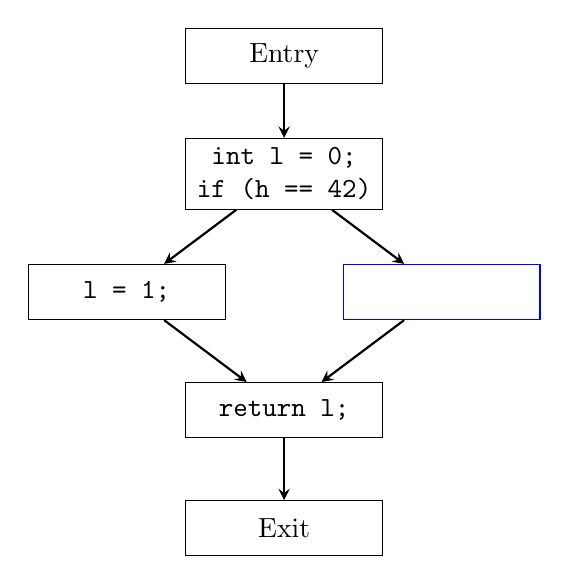
\begin{tikzpicture}
                \tikzstyle{node} = [rectangle, minimum width=2.5cm, minimum height=.7cm, text centered, draw=black, node distance=1.5cm]
                \tikzstyle{arrow} = [thick,->,>=stealth]
                
                \node (entry) [node] {Entry};
                \node (b1) [node, below of=entry, align=center] {\texttt{int l = 0;} \\ \texttt{if (h == 42)}};
                \node (b2) [node, below of=b1, xshift=-2cm] {\texttt{l = 1;}};
                \node (b22) [node, below of=b1, xshift=+2cm, draw = blue] {};
                \node (b3) [node, below of=b2, xshift=+2cm] {\texttt{return l;}};
                \node (exit) [node, below of=b3] {Exit};

                \draw [arrow] (entry) -- (b1);
                \draw [arrow] (b1) -- (b2);
                \draw [arrow] (b1) -- (b22);
                \draw [arrow] (b2) -- (b3);
                \draw [arrow] (b22) -- (b3);
                \draw [arrow] (b3) -- (exit);
            \end{tikzpicture}
        \caption{Control Flow Graph\\The highlighted node was inserted to split a critical edge.}
        \label{fig:cfg}
    \end{subfigure}\hfill
    \begin{subfigure}[t]{.45\textwidth}
        \centering
        \begin{tikzpicture}
            \tikzstyle{node} = [ellipse, minimum width=2.5cm, minimum height=.7cm, text centered, draw=black, node distance=2cm]
            \tikzstyle{arrow} = [thick,->,>=stealth]
            
            \node (b1) [node] {\texttt{int l = 0;}};
            \node (b2) [node, below left of=b1] {\texttt{h == 42}};
            \node (b3) [node, below of=b2] {\texttt{l = 1;}};
            \node (b4) [node, below right of=b3] {\texttt{return l;}};

            \draw [arrow] (b1) -- (b4);
            \draw [arrow, blue] (b2) -- (b3);
            \draw [arrow] (b3) -- (b4);
        \end{tikzpicture}
        \caption{Program Dependence Graph\\The black edges are data dependencies, while blue edges show control dependencies}
        \label{fig:pdg}
    \end{subfigure}
    \caption{Different graph representations for the program snippet in \ref{fig:ifEx}}
\end{figure}


\section{Program Slicing}

\com{put in new section: static techniques? could also include some stuff about what nildumu does}

Slicing is a technique used to find those sections of a program, that are influenced by or in other cases influence a given location in the program \cite{weiser81}.
This location is called the \emph{slicing criterion} and is a tuple $\langle s, v \rangle$ of a program statement $s$ and a variable $v$.
A \emph{backward slice} contains all statements that the slicing criterion has data or control dependencies to, i.e. statements that influence the behaviour of the program at point $s$. Figure \ref{fig:slice} shows an example of a backward slice.
A \emph{forward slice} is the subset of program statements that are influenced by the slicing criterion.

Computing a program slice can be efficiently done using the PDG of the given program. Since all dependencies are explicitly represented as edges, the computation of a program slice is reduced to a reachability problem \cite{ottenstein84}. Horwitz \cite{horwitz88sdg} noted that interprocedural slices could be computed similarly using system dependence graphs.

Tools like JOANA use slicing techniques on system dependence graphs to analyse the information flow in programs and give non-interference guarantees where possible \cite{hammer09}.

\begin{figure}
    \centering
    \begin{minipage}{.4\textwidth}
        \begin{algorithm}[H]
            \hspace*{\algorithmicindent} \textbf{Input} h: int \\
            \hspace*{1em}
            \begin{algorithmic}
                \State $i: int \leftarrow 0$
                \State $sum: int \leftarrow 0$
                \State $product: int \leftarrow 1$
                \While{$i \leq h$}
                    \State $sum \leftarrow sum + i$
                    \State $product \leftarrow product * i$
                    \State $i++$
                \EndWhile
                \State $\mathtt{print}(sum)$
                \State $\mathtt{print}(product)$
            \end{algorithmic}
        \end{algorithm}
    \end{minipage}
    \hfill
    \begin{minipage}{.4\textwidth}
        \begin{algorithm}[H]
            \hspace*{\algorithmicindent} \textbf{Input} h: int \\
            \hspace*{1em}
            \begin{algorithmic}
                \State $i: int \leftarrow 0$
                \State $sum: int \leftarrow 0$
                \State $\color{white} product: int \leftarrow 1$
                \While{$i \leq h$}
                    \State $sum \leftarrow sum + i$
                    \State $\color{white} product \leftarrow product * i$
                    \State $i++$
                \EndWhile
                \State $\color{blue} \mathtt{print}(sum)$
                \State $\color{white} \mathtt{print}(product)$
            \end{algorithmic}
        \end{algorithm}
    \end{minipage}
    \caption{The right side shows a backward slice of the function on the left for the slicing criterion $\langle \mathtt{print}(sum), sum \: \rangle$}
    \label{fig:slice}
\end{figure}


\section{Model Counting}

Given a propositional formula $F$, the model counting problem (\#SAT) is the problem of finding the number of distinct variable assignments for $F$, for which $F$ evaluates to true \cite{biere09}. So the solution for the formula shown in  \ref{fig:satEx} is \#F = 3, with the only non-fulfilling variable assignments being $\{ x = \mttt, y = \mfff\}, \{x = \mttt, y = \mttt\}$ and  $\{x = \mfff, y = \mfff\}$.

\#SAT is a generalization of the SAT problem and falls into the \#P-complete complexity class, as demonstrated by Valiant in \cite{valiant79}.

Early exact model counting techniques, such as \cite{birnbaum99}, or the well-known tool sharpSAT \cite{thurley06} use a DPLL-style exploration of the solution space. Another class of model counters instead employ complex transformations to turn the given CNF formula into a different representation, which makes model counting a far easier problem. Common are transformations into \emph{binary decision diagrams} (\td{citation!}) or \emph{deterministic, decomposable negation normal form} \cite{darwiche04}.

\paragraph*{Approximate Model Counting}
State-of-the-art exact model counters scale to a couple of hundred variables.  This limit can be pushed to around 1,000 variables if we allow approximate solutions \cite{biere09}.
The first approximate \#SAT algorithm for DNF formulas was introduced by Luby and Karp in \cite{karp89} used Monte-Carlo techniques. This approach was extended to work on CNF formulas by Chakraborty, Meel and Vardi in \cite{chakraborty13}. Both procedures fall under category of $(\epsilon, \delta)$-counters: for $0 < \epsilon, \delta \leq 1$, the approximated solution $\#F_{approx}$ to the true solution of the problem \#F, lies in the interval $[(1 + \epsilon)^{-1} \#F, \: (1 + \epsilon) \#F]$ with a probability of $1 - \delta$ \cite{karp89,chakraborty13}.

\begin{figure}
    \centering
    $F := x \lor \lnot y$
    \caption{Propositional formula with 2 variables}
    \label{fig:satEx}
\end{figure}

\paragraph*{Projected Model Counting}
Given a set of propositional variables $\mathcal{V}$ and a propositional formula $F$ over $\mathcal{V}$, projected model counting (\#$\exists$SAT) is the problem of finding the number of assignments to a set of priority variables $\mathcal{P} \subseteq \mathcal{V}$, such that the assignment can be extended to an assignment over $\mathcal{V}$ that fulfills $F$. Considering the example from \ref{fig:satEx} and a priority set $\mathcal{P} = \{x\}$, the number of projected models is 2, with both possible assignments of $x$ being extendable to a fulfilling assignment over all variables by setting $y = \mfff$.

The problem is introduced by Aziz et.al. in \cite{aziz15}, along with a discussion of approaches to solve \#$\exists$SAT. \td{finish}

% Model Counting
% Complexity
% Hashing-based approaches
% Application to CNF
% (\epsilon, \delta) approximation / "Probably Approximately Correct"

%%% relevant for this section
% The Complexity of Enumeration and Reliability Problems (Valiant '79) -- \cite{valiant79}
% A scalable approximate model counter (chakraborty '13) -- \cite{chakraborty13}

\chapter{Design and Implementation}\label{sec:impl}

As outlined in section \ref{sec:relWork}, there have been attempts at using symbolic execution and model counting to measure how much information a program can leak. In many of these works, there have been attempts to mitigate the problems that are caused by path explosion in input programs and the computational limits of state of the art model counters. These attempts include using approximate model counting instead of a precise calculation (\cite{biondi18, chu19}) or transformations of SAT formulas into easier to handle representations (\cite{klebanov13}). We have not yet seen an attempt to use static (Q)IFC techniques to reduce complexity at the time of formula creation. \com{besser in related work? oder sogar intro?}

The analysis we will present in the following chapter combines static and dynamic approaches to the QIFC problem. 

We will run a static pre-processing to identify program parts that are critical to the flow of information and restrict the subsequent dynamic analysis to those parts.

The dynamic analysis finds and examines possible execution paths using symbolic execution and evaluates and information flow along these paths through an approximate model counter, similar to the techniques we have seen in \cite{klebanov13, biondi18, chu19}.
If during the analysis, the generated boolean predicates are still too complex to be evaluated by a model counter, out tool will split the program into segments and separately, either statically or dynamically, analyze each segment and combine the results for an overall estimation of the programs channel capacity.

The analysis is integrated in an interpreter that will execute the program for a given input and, additionally to the channel capacity, will give estimations for the size of the indistinguishability class of the given input.

\td{which guarantees does our analysis give?}

% input program:
% - javac --> bytecode
% working on CFG + SSA form

\section{Input Programs and Program Representation}\label{sec:inputLang}

Input programs are written in a variant of the \texttt{while}-language with Java-like syntax, that contains the following control structures, using their standard semantics:
\begin{itemize}
    \setlength\itemsep{0em}
    \item sequential composition
    \item assignments
    \item \texttt{if}-statements
    \item \texttt{while}-statements
    \item \texttt{break}-statements
    \item function calls (with return values)
\end{itemize}
All variables are signed integers of a fixed width $w$. The right hand side of an assignment is an expression that uses the standard arithmetic and bitwise boolean operators. Boolean expressions used in \texttt{while}- and \texttt{if}-statements are defined in the standard way.

We will denote secret inputs as $h_i$, constant values as $n_i$ and other program variables as $x_i$. The set of all input variables for a program will be denoted as \In and the set of all possible input sets is written as \allIn. A variable can be leaked to a public output channel via the special function \texttt{print}. We assume that all program executions terminate. More specifically, we assume that they terminate normally, without throwing any exceptions.

To analyze the input program \p, we use the program's functions' control flow graphs (CFG) in static single assignment (SSA) form.

\begin{itemize}
    \item \note{execution values: represent actual value during execution}
    \item \note{represented as bit vectors (two's complement}
    \begin{itemize}
        \item integers: width n
        \item booleans: width 1
    \end{itemize}
    \item \com{specify relationship between valueDeps and execVal}
\end{itemize}

\begin{definition}[Execution Value]
The function maps a program value to the number that was assigned during a particular execution. If in this execution, the value remains undefined, because the corresponding assignment instruction wasn't executed, the function will return $\bot$.
    \begin{center}
        $exec_{\mI, p}: \val_p \longrightarrow \{0, 1\}^n \cup \{\bot\}$
    \end{center}
The function is parameterized by the input \p and the set of program inputs \I, which determine the particular execution of \p that is evaluated.
\end{definition}

\begin{definition}[Value Dependencies]

    
\end{definition}

\section{Basic Analysis Design}

\begin{itemize}
    \item \note{approach: symbolic execution}
    \item \note{data + cf dependencies represented as boolean formulas}
    \item \com{define set of boolean formulas, \ttt, \fff, operators etc.}
\end{itemize}

We use propositional logic to track the way that information about the secret inputs flows through the program. Each program value is interpreted as a bit vector, where each bit is associated with a propositional formula that encodes how the state of the bit is dependent on the secret inputs. We will use subscript indices to access the i-th bit of a program value or the i-th element of a vector respectively. The bitwidth of a value \texttt{x} will be denoted as $width(\mathtt{x})$.

\begin{definition}[Independent Set]
    Let \texttt{H} be the set of input values of \pp.
    \begin{center}
        $\var_p := \bigcup\limits_{\mathtt{h} \in \mathtt{H}} \{h^j | 0 \leq j \leq width(\mathtt{h})\}$
    \end{center}
    The values of a program's input parameters are not dependent on any other value in the program. We define the set $\var_p$, that contains a propositional variable for each input bit. Every other value of \p is either constant or can be described by a propositional formula over $\var_p$.
\end{definition}

\textbf{\note{Implicit information flow (CF dependencies)}}

\begin{itemize}
    \item \note{Associate each block w/ a boolean formula that evaluates to true <==> block is executed in the specific execution}
    \item \note{a block is executed iff one of its predecessors is executed and if the jump comdition from that predecessors evaluates to true}
    \item \com{Function for accessing condition of a conditional kump at the end of block -->} \question{necessary?}
    \item \question{`Abbildungsvorschrift' nötig?}
    \item \com{imDep: bblock -> formula -- f === wahr <--> b wird ausgeführt}
\end{itemize}

% define implicit leakages
\paragraph{Implicit Information Flow}

% TODO: better description for the case conditions
% TODO: check if this is even correct lol
% TODO: is knowledge the right word to use here?
% TODO: find better name for function than Phi

\paragraph{Explicit Knowledge Function}

% map + semantics for finding implicit leakage

\section{Increasing Efficiency through Static Pre-Processing}
\begin{itemize}
    \item "Konstantenfaltung" auf Bitebene
    \item Backward-Slice des Ausgabewerts, nicht enthaltene Werte müssen nicht analysiert werden
    \item Backward-Slice von Konstanten Werten --> Werte, die die Ausgabe beeinflussen und Abhängigkeiten dadurch immer durch konstanten Wert fließen müssen nicht analysiert werden
\begin{itemize}
    \item kann mitberücksichtigt werden, wenn man vor dem "Ausgabe-Backward-Slice" alle Abhängigkeiten von konstanten Werten entfernt 
\end{itemize}
\end{itemize}

\section{Handling Loops, Recursion and Function calls}

\section{Combining static and dynamic analyses to estimate channel capacity}
\textbf{Goal:}
\begin{itemize}
    \item channel capacity c := number of distinct program outputs
    \item c large --> much leakage
    \item c small --> little leakage
\end{itemize}
Consider program w/ single loop. Precisely computing channel capacity might be infeasible due to too many possible execution paths through the loop

\begin{itemize}
    \item Define unrolling limit n
    \item Compute SAT formula $cond_n$ where $cond_n(h) == true$ iff input h leads to more than n loop iterations
    \item if $SAT(cond_n)$ we cannot analyze the loop in a purely dynamic manner
    \item \textbf{Switch to an analysis in parts}
\end{itemize}

\textbf{Analysis in parts:}
\begin{itemize}
    \item Let c = true channel capacity of the program
    \item divide program into 3 parts: $p_b$ - before loop, $p_l$ - loop body, $p_a$ - after loop
    \item compute channel capacities for all 3 parts separately: $k_b, k_l, k_a$
    
    \begin{itemize}
        \item take into account constant bits in result from previous program part for inputs for next part
        \item for loop part: only analyze a single loop iteration
        \item \com{Could be done with dynamic or static analysis}
    \end{itemize}
    
    \item each analysis (except the first) overapproximates the possible inputs for the program section --> computed channel capacities possibly larger than they actually are --> sound upper limit for leakage
    \item $c \leq k_b, k_l, k_a \implies c \leq \min{k_b, k_l, k_a}$
    \item \com{Correction: Implicitly assumes that loop is executed at least once}
    \begin{itemize}
        \item Use model counter to estimate number of inputs that would not enter the loop --> $k_n$
        \item worst case: these are all different to what the loop outputs are
        \item update $k_l += k_n$
        \item instead of $p_l$, estimate channel capacity of if (cond) $p_l$ else skip --> all inputs that don't enter the loop (produce outputs that are accounted for in $k_n$ will lead to the same output in $p_l$; avoid counting them double)
        \item \com{instead of $p_l$ directly, compute channel capacity of \\ \texttt{if (cond) res = loopBody else res = h return res}}
        \item set p := $loopBody^n$ if (loop cond) loopBody else return $\bot$ to find channel capacity for program runs that execute loop more than n times
        \item for executions that execute loop less than n times: count loop iterations as part of $p_b$
    \end{itemize}
    \item \com{all partial analyses could be done either statically or dynamically}
        \begin{itemize}
        \item \question{when to use what?}
        \item \question{shouldn't purely dynamic analysis be feasible for all program parts here since we `eliminated' the many loop iterations?}
        \item \note{might still not be possible bc loop might contain another loop, or recursive function, etc. --> further segmentation necessary}
        \item number of segments that need to be analysed separately explodes
        \item switch to static analysis when num. of segments gets too large, before then do everything dynamically to get more precise estimations
        \item \textbf{How to decide when to do what?}
        \begin{itemize}
            \item for each segment: keep track of `segmentation depth' $s$
            \item define segmentation limit $\hat{s}$
            \item if $s >= \hat{s}$, but segment can still not be feasibly analysed in a dynamic manner, switch to static 
        \end{itemize}
    \end{itemize}
    
    
    \item \question{How do we know, when to further partition the program?}
    \begin{itemize}
        \item number of loop iterations that possibly happen
        \item width of SAT formulas generated up until this point --> number of operands, number of nodes, number of literals
        
    \end{itemize}
     \item \com{\textbf{Alternative approach:}}
    \begin{itemize}
        \item use same method as for estimation of indistinguishability set
    \end{itemize}
    
\end{itemize}

\note{while (i < secret) { if (i > 64) {i = 100; break;} i++}}

\section{Integration with Interpreter}
\begin{itemize}
    \item channel capacity --> measures leakage in terms of the number of different outputs a program can produce
    \item even if there are only 2 different outputs, if one of those outputs can only be the result of one input, then the attacker will learn the whole secret
    \item interesting for user to know the number of inputs to the program that will produce the same output as the user's execution did --> `indistinguishability set' D
    \item D large --> leakage small
    \item D small --> leakage big
    \item precise computation of $|D|$ infeasible, we need to estimate
    \begin{itemize}
        \item Problem: loops + recursive calls produce SAT formulas that are too big to handle efficiently
    \end{itemize}
\end{itemize}

\textbf{Underapproximation of $|D|$ --> finding max amount of leakage for this run}\\
Consider program that contains a loop
\begin{itemize}
    \item not feasible to precisely analyse all possible numbers of loop iterations
    \item choose unrolling limit $n$
    \item get SAT formula $cond_n: cond_n == true$ iff input needs less than n iterations
    \item only seek candidates for $D$ among inputs that require less than $n$ loop iterations by adding $\land cond_n$ to Model Count formula --> $D_u$
    \item definitely $D_u \subseteq D$, so $|D_u|$ is sound upper bound for leakage
\end{itemize}
More precise approximation? So far we haven't considered executions ith $>n$ loop iterations at all
\begin{itemize}
    \item 
\end{itemize}

\textbf{Overapproximation of $D$ --> finding min amount of leakage for this run}
Consider program that contains a loop
\begin{itemize}
    \item not feasible to precisely analyse all possible numbers of loop iterations
    \item choose unrolling limit $n$
    \item get SAT formula $cond_n: cond_n == true$ iff input needs less than n iterations (same as above)
    \item formula that describes result of loop for $< n$ iterations: $b_{<}$
    \item introduce new vars: $v_>$
    \item set loop result as $cond_n ? b_{<} : v_>$ --> use that for model counting to find set $D_o$
    \item allows inputs with more than n iterations to produce arbitrary results from the loop
    \item every result that might actually occur is contained, but also one's that are not actually possible --> $D \subseteq D_o$, so $|D_o|$ is sound lower bound for leakage
\end{itemize}

\com{Possible to use a form of static analysis for estimation of indistinguishability set?}

\begin{itemize}
    \item static analyses determine the number of distinct outputs, not the size of the indistinguishability set
    \item \question{can we manipulate the program s.t. the number of distinct outputs is the same as the size of $D$?}
    \item desired output: $o$
    \item set $p_new(h)$ := res = p(h) if (res == o) return h else return $\bot$
    \item every input that is not part of $D$ gets mapped to the same output
    \item result will be overestimation of $|D|$ --> gives us \textbf{lower bound of leakage}
    \item can only work on the whole program, not on segments (would be a possible underapproximation of $D$ for middle segments) --> under- and overapproximating at the same time is not good...
    \item \com{underapproximation if we change (res == o) to (res != o) ??}
\end{itemize}

\section{Implementation}
\chapter{Evaluation}\label{sec:eval}

\begin{itemize}
    \item \note{compare execution time with and without static preprocessing}
    \item \note{compare size of mc formula with and without static preprocessing}
\end{itemize}
\chapter{Fazit und Ausblick}\label{sec:conclusion}


\bibliographystyle{ieeetr}
\bibliography{bib}

\begin{otherlanguage}{ngerman}
\chapter*{Erklärung}
\pagestyle{empty}

  \vspace{20mm}
  Hiermit erkläre ich, \theauthor, dass ich die vorliegende Bachelorarbeit selbst\-ständig
verfasst habe und keine anderen als die angegebenen Quellen und Hilfsmittel
benutzt habe, die wörtlich oder inhaltlich übernommenen Stellen als solche kenntlich gemacht und
die Satzung des KIT zur Sicherung guter wissenschaftlicher Praxis beachtet habe.
  \vspace{20mm}
  \begin{tabbing}
  \rule{4cm}{.4pt}\hspace{1cm} \= \rule{7cm}{.4pt} \\
 Ort, Datum \> Unterschrift
  \end{tabbing}
\end{otherlanguage}

\chapter*{Danke}
\pagestyle{empty}

Ich danke meinen Eltern, meinem Hund und sonst niemandem.

\pagestyle{fancy}
\appendix

\chapter{Proof for Equation \ref{eq:ev}}\label{ch:evProof}

Let $p$ be a deterministic program, with input \In and output \Out. Let $\mathcal{L}$ be the set of possible outputs.

\begin{align*}
    cc(p) &:= H_\infty(\mIn) - H_\infty(\mIn \: | \: \mOut) \\
    &= H_\infty(\mIn) - \sum\limits_{l \in \mathcal{L}} P[L = l]\: H_\infty(\mIn \: | \: \mOut = l) \\
    &= H_\infty(\mIn) - \sum\limits_{l \in \mathcal{L}} P[L = l]\: (-L_{dyn}(p, l) + H_\infty(\mIn)) \\
    &= H_\infty(\mIn) - \sum\limits_{l \in \mathcal{L}} P[L = l]\: H_\infty(\mIn) + \sum\limits_{l \in \mathcal{L}} P[L = l]\: L_{dyn}(p, l) \\
    &= \sum\limits_{l \in \mathcal{L}} P[L = l] \: L_{dyn}(p, l) \\
    &= \mathbb{E}(L_{dyn}(p,l))
\end{align*}

The equality in the second line results from the definition of $H( \mIn \: |\: \mOut)$, which is given in \cite{smith09}. All other steps in the proof use the definitions given in chapter \ref{ch:measures}.

\chapter{Proof of Theorem \ref{thm:equiv}}\label{ch:proofEquiv}

In this chapter we present a proof for the correctness of theorem \ref{thm:equiv}. We prove the correctness of the theorem for the programs addressed in section \ref{sec:design}, i.e. programs without loops, function calls and arrays.

The proof is presented in the following steps:
\begin{enumerate}
    \setlength\itemsep{0em}
    \item We show that theorem \ref{thm:equiv} holds for programs without diverging control flow
    \item proof correctness of edge annotations $follow(e)$
    \item proof correctness of $exec(b)$
    \item proof correctness of cf stuff
\end{enumerate}

\paragraph{Linear Programs}
Let $p$ be a program with linear control flow and let $v \in \val_p$ be an arbitrary value in $p$, that is defined by the statement $v \leftarrow e$.

Let $v_h := \llbracket p \rrbracket_h(v)$ be the bit vector of the execution value of $v$ for the execution with input an arbitrary but fixed input $h$. The dependency vector of $v$ is defined as $dVec(v) := \mathcal{E}(e)$. We show that $\forall 0 \leq i < w: \mathcal{V}_h(\mathcal{E}(e))^i \iff v_h^i$.

Distinction of cases for $e$:
\begin{enumerate}
    \item $e := n, \quad n \in \mathbb{Z} \implies v_h = bv(n)$\\
    Per definition $\mathcal{E}(e) = bv(n)$. Thus $\forall 0 \leq i < w: \mathcal{V}_h(\mathcal{E}(e))^i \iff v_h^i$
    
    
    \item $e := \mIn \implies v_h = bv(h)$\\
    Per definition $\mathcal{E}(e) = \var(h)$ and $\mathcal{V}_h(\var(h)) = bv(h)$. Thus\\ $\forall 0 \leq i < w: \mathcal{V}_h(\mathcal{E}(e))^i \iff v_h^i$
    
    
    \item $e := v', \quad v' \in \val_p \implies v_h = \llbracket p \rrbracket_h (v')$\\
    Assumption: Behauptung erfüllt für $v' \implies$ Behauptung gilt nach Voraussetzung
    
    \item 
    
\end{enumerate}


\end{document}
